
\chapter{Complex Numbers}

The complex numbers arose through the study of polynomials, but there is hardly an area of modern mathematics where they are not of use, with applications stretching from number theory to geometry to quantum mechanics.


\section{Defining the Complex Numbers}

We are going to start right at the beginning, though some familiarity with complex numbers is assumed.
We will construct the set of complex numbers, denoted by $\C$, from the real numbers $\R$ by adjoining an element $i$ with the property that $i^2 = -1$.

\begin{definition}[Complex Numbers]
	A \vocab{complex number} is a number $z \in \C$ of the form $z = x + yi$ with $x, y \in \R$ such that $i^2 = -1$. 
	
	We call $x = \re(z)$ the \vocab{real part}, and $y = \im(z)$ the \vocab{imaginary part} of $z$.
\end{definition}

The reals are a subset of the complex numbers, as for $x \in \R$, we have $x + 0i \in \C$. 

\subsection{Basic Operations}

With the complex numbers defined, we have to come up with some things to do with them.
We can add, subtract, multiply and divide complex numbers in a sensible way, and indeed they form a \emph{field} (we will elaborate on this later).

\begin{definition}[Basic Operations in $\C$]
	Let $z_1 = x_1 + y_1 i$ and $z_2 = x_2 + y_2 i$ be two complex numbers. Then we define \vocab{addition} and \vocab{multiplication} as
	\begin{align*}
		z_1 + z_2 &= (x_1 + x_2) + (y_1 + y_2)i,\\
		z_1 \times z_2 &= (x_1 x_2 - y_1 y_2) + (x_1 y_2 + x_2 y_1)i.
	\end{align*}
\end{definition}

We can see from this definition that the operation of multiplication respects our original requirement that $i^2 = -1$. From these definitions we can also immediately define \vocab{subtraction} and \vocab{division} as the inverse operations of these, with
\begin{align*}
	z_1 - z_2 &= (x_1 - x_2) + (y_1 - y_2)i \\
	\frac{z_1}{z_2} &= \frac{x_1 + y_1 i}{x_2 + y_2 i} \cdot \frac{x_2 - y_2i}{x_2 - y_2 i} = \left(\frac{x_1y_1 + x_2 y_2}{x_2^2 + y_2^2}\right) + \left(\frac{x_2y_1 - x_1 y_2}{x_2^2 + y_2^2}\right)i.
\end{align*}

From the definitions of addition and multiplication, it is clear that both operations are commutative and associative. Indeed, as we also have inverse operations, the complex numbers form groups.

\begin{proposition}[$\C$ is a Group]
	$\C$ with the operation $+$ is an abelian group with identity $0$, and $\C \backslash \{0\}$ with the operation $\times$ is an abelian group with identity $1$.
\end{proposition}
\begin{proof}[Proof Sketch]
	Check definitions and verify that $+$ and $\times$ are indeed associative.
\end{proof}

Another useful operation is the \emph{complex conjugate}. 

\begin{definition}[Complex Conjugation]
  For a complex number $z = x + iy$, we define its \vocab{complex conjugate} to be $\overline{z} = z^* = x - iy$.
\end{definition}

Complex conjugation allows us to extract the real and imaginary parts of a complex number, with
$$
\re(z) = \frac{z+ \overline{z}}{2}, \quad \text{and} \quad \im(z) = \frac{z - \overline{z}}{2i}.
$$
For complex numbers $z_1$ and $z_2$, we have $\overline{(\overline{z})} = z$, $\overline{z_1 + z_2} = \overline{z_1} + \overline{z_2}$ and $\overline{z_1 z_2} = \overline{z_1} \cdot  \overline{z_2}$.

\begin{aside}{Aside: The History of Complex Numbers}

The complex numbers arose through the study of polynomials, and their serious study really began in the study of the \emph{cubic} polynomials of the form\footnote{This form of a cubic equation is a `depressed', and any general cubic can be expressed in this form.}
$$
x^3 - 3px - 2q = 0.
$$
The sixteenth century mathematicians del Ferro, Tartaglia and Cardano discovered that this equation could be solved explicitly, with the result being published in Cardano's 1545 work \emph{Ars Magna} (where he mentioned del Ferro as a first author, and noted that Tartaglia had independently found the same result).
The solution they had obtained was
$$
x = \sqrt[3]{q + \sqrt{q^2 - p^3}} + \sqrt[3]{q - \sqrt{q^2 - p^3}}.
$$
For example, for the cubic $x^3 - 12x - 20$ we obtain the solution $x = \sqrt[3]{16} + \sqrt[3]{2}$. 

Some 30 years later, Rafael Bombelli discussed one particular cubic in his work \emph{l'Algebra}. He looked at $x^3 - 15x - 4 = 0$.
One might observe (through mere trial and error) that $x = 4$ is a solution, but using Cardano's formula, we obtain the solution
$$
x = \sqrt[3]{2 + \sqrt{-121}} + \sqrt[3]{2 - \sqrt{-121}}.
$$
Indeed, Bombelli noticed this and gave an explanation for how these two solutions were essentially the same, even with the presence of the rather puzzling term $\sqrt{-121}$.
His explanation essentially began by noting that if we wrote $\sqrt{-121} = 11i$, then we could find that
\begin{align*}
	\sqrt[3]{2 + \sqrt{-121}} &= 2 + ni \\
	\sqrt[3]{2 - \sqrt{-121}} &= 2 - ni,
\end{align*}
and adding would then result in $2 + ni + 2 - ni = 4$, our other solution.

Inherent in this explanation was an expectation that this $i$ would obey many of the same rules of arithmetic that we would expect of, say, a real number. After this work, contributions from mathematicians such as Descartes, Wallis, de Moivre, Euler, Wessel, Argand, Hamilton, Gauss, Cauchy and many others began to build up a rich theory of the complex numbers, later developing the field of complex analysis, all centered on this construction of some $i$ with the property that $i^2 = -1$. 

\end{aside}

Looking again at the solutions to polynomials it turns out that the complex numbers are sufficient to solve \emph{every} polynomial equation. This result is known as the `Fundamental Theorem of Algebra', and was proved in the 18th century. We will use it frequently in this course, but you will have to wait until a later course to see a proof.
\begin{theorem}[Fundamental Theorem of Algebra]
Let $p(z)$ be a polynomial of degree $n \geq 1$ with complex coefficients. Then $p(z) = 0$ has precisely $n$ (not necessarily distinct) complex roots, counted with multiplicity. 
\end{theorem}

\subsection{The Argand Diagram}

There is a geometric way to interpret complex numbers and the way that they operate. We can plot a complex number $z = x + yi$ on the \vocab{Argand diagram} or \vocab{complex plane} by associating it with a point $(x, y)$. We call the $x$ axis the `real' axis, and the $y$ axis the `imaginary' axis.

\begin{center}
  \begin{tikzpicture}
    \draw [->] (-1, 0) -- (3.5, 0) node [right] {$\re$};
    \draw [->] (0, -1) -- (0, 2.75) node [above] {$\im$};
	\draw [->] (0, 0) -- (2.5, 1.7) node [anchor=south west] {$x + yi$} node [pos=0.5, above] {$r$} node [pos=0.3, below] {$\theta$};
    \draw [dashed] (0, 1.7) node [left] {$y$} -- (2.5, 1.7) -- (2.5, 0) node [below] {$x$};
  \end{tikzpicture}
\end{center}

From the complex number written $z= x + yi$, we can plot it in rectangular coordinates. However, it can also be useful to plot it using polar coordinates. With this in mind, we introduce some useful 
definitions.

\begin{definition}[Modulus]
	For a complex number $z = x + yi$, we define its \vocab{modulus} to be $r = |z|$ such that $r \geq 0$ and $r^2 = |z|^2 = x^2 + y^2$.
\end{definition}

Indeed, this definition matches the distance from the origin of the Argand diagram to the point $(x, y)$.

\begin{definition}[Argument]
	For a non-zero complex number $z$, we define its \vocab{argument} to be $\theta = \arg(z)$, a real number such that $z = r(\cos \theta + i \sin \theta)$. We say this is the \vocab{polar form} of $z$.
\end{definition}

From this, we get that for $z = x + yi$,
$$
\cos \theta = \frac{x}{\sqrt{x^2 + y^2}}, \quad \sin \theta = \frac{y}{\sqrt{x^2 + y^2}}, \quad \text{and} \quad \tan \theta = \frac{y}{z}.
$$

An important point to note is that $\arg(z)$ is only defined up to multiples of $2 \pi$, as mapping $\theta \mapsto \theta + 2\pi$ leaves $z$ unchanged. So, to make $\theta$ unique (which is often useful), we typically restrict its range. For example, if we restrict $- \pi < \theta \leq \pi$, we get the \vocab{principle value} of $\theta$.

Using the Argand diagram, there is a geometric 
way to define addition, multiplication and complex conjugation. Addition and subtraction correspond to parallelograms constructed as shown.

\begin{center}
	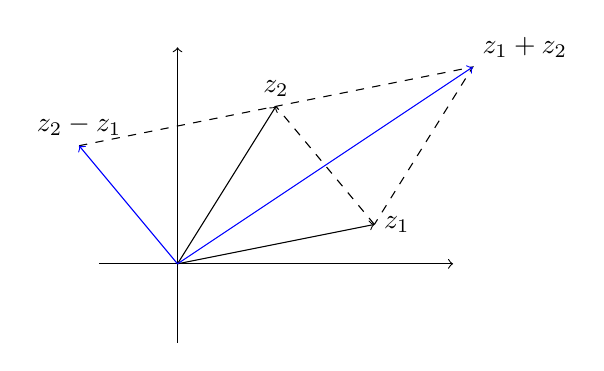
\begin{tikzpicture}
	  \draw [->] (-1, 0) -- (3.5, 0) node [right] {$\re$};
	  \draw [->] (0, -1) -- (0, 2.75) node [above] {$\im$};
	  \draw [->] (0, 0) -- (2.5, 0.5) node [anchor=west] {$z_1$};
	  \draw [->] (0, 0) -- (1.25, 2.0) node [anchor=south]{$z_2$};
	  \draw [dashed] (-1.25, 1.5) -- (3.75, 2.5) node [anchor=south west] {$z_1 + z_2$}  -- (2.5, 0.5);
	  \draw [dashed] (2.5, 0.5) -- (1.25, 2.0);

	  \draw [->, color=blue] (0, 0) -- (3.75, 2.5); 
	  \draw [->, color=blue] (0, 0) -- (-1.25, 1.5) node [color=black, anchor=south] {$z_2 - z_1$};
	\end{tikzpicture}
  \end{center}

  Complex conjugation corresponds to reflection in the real axis.

  \begin{center}
	\begin{tikzpicture}
	  \draw [->] (-1, 0) -- (3.5, 0) node [right] {$\re$};
	  \draw [->] (0, -2) -- (0, 2) node [above] {$\im$};
	  \draw [->] (0, 0) -- (2.5, 1.4) node [anchor=south west] {$z = x + yi$};
	  \draw [color=blue, ->] (0, 0) -- (2.5, -1.4) node [color=black, anchor=south west] {$\overline{z} = x - yi$};
	  \draw [dashed] (2.5, 1.4) -- (2.5, -1.4);
	\end{tikzpicture}
  \end{center}

  Multiplication is slightly more complex. If we have two complex numbers in polar form, $z_1 = r_1 (\cos \theta_1 + \sin \theta_1)$ and $z_2 = r_2 (\cos \theta_2 + \sin \theta_2)$, then $z_1 z_2 = r_1 r_2 (\cos \theta_1 + \theta_2 + \sin \theta_1 + \theta_2)$.
  This gives the following.

  \begin{proposition}[Moduli Multiply and Arguments Add]
	  For complex numbers $z_1$ and $z_2$, we have $\arg(z_1 z_2) = \arg(z_1) + \arg(z_2)$ and $|z_1 z_2| = |z_1| \cdot |z_2|$.
  \end{proposition}

  This is shown in the diagram below.

  \begin{center}
	\begin{tikzpicture}
	\coordinate (origin) at (0,0);
	\coordinate (one) at (1.0, 0.0);
	\coordinate (im) at (0.0, 1.0);
	\coordinate (z1) at (3.0, 1.0);
	\coordinate (z2) at (1.5, 1.5);
	\coordinate (z) at (2, 4);

	% draw axes
	\draw [->] (-1, 0) -- (3.5, 0) node [right] {$\re$};
	\draw [->] (0, -1) -- (0, 2.75) node [above] {$\im$};

	% draw vectors
	\draw [->] (origin) -- (z1) node [anchor=south west] {$z_1$};
	\draw [->] (origin) -- (z2) node [anchor=south west] {$z_2$};
	\draw [->] (origin) -- (z) node [anchor=south west] {$z_1 z_2$} node [pos=0.85, anchor=east] {$|z_1|  |z_2|$};

	\pic [draw, ->, angle eccentricity=1.2, angle radius=1.75cm, color=blue] {angle = one--origin--z1};
	\pic [draw, ->, angle eccentricity=1.2, angle radius=1.75cm, color=purple] {angle = z1--origin--z};

	\pic [draw, ->, angle eccentricity=1.2, angle radius=1.25cm, color=purple] {angle = one--origin--z2};
	\pic [draw, ->, angle eccentricity=1.2, angle radius=1.25cm, color=blue] {angle = z2--origin--z};
	\end{tikzpicture}
  \end{center}

To see how useful a geometric perspective can be, consider the following result.

\begin{proposition}[Triangle Inequality]
	For complex numbers $z_1$ and $z_2$, $|z_1 + z_2| \leq |z_1| + |z_2|$.
\end{proposition}
\begin{proof}[Algebraic Proof]
	We have $|z_1 + z_2|^2 = (z_1 + z_2)\overline{(z_1 + z_2)} = |z_1|^2 + z_1 \overline{z_2} + \overline{z_1} z_2 + |z_2|^2$, so it suffices to show that $z_1 \overline{z_2} + \overline{z_1} z_2 \leq 2 |z_1| |z_2|$. To show this, we have
	\begin{align*}
		z_1 \overline{z_2} + \overline{z_1} z_2 &\leq 2 |z_1| |z_2| \\
\iff 	\frac{z_1 \overline{z_2} + \overline{z_1 \overline{z_2}}}{2} &\leq |z_1| |\overline{z_2}| \\
\iff \re(z_1 \overline{z_2}) &\leq |z_1 \overline{z_2}|,
	\end{align*}
	which is true. 
\end{proof}

Now put everything on an Argand diagram and stare at it for a minute.


\begin{center}
	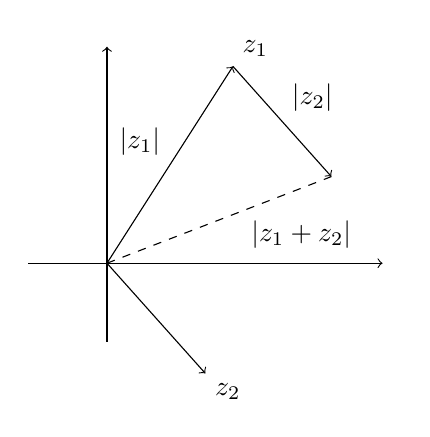
\begin{tikzpicture}
	\coordinate (origin) at (0,0);
	\coordinate (one) at (1.0, 0.0);
	\coordinate (im) at (0.0, 1.0);
	\coordinate (z1) at (1.6, 2.5);
	\coordinate (z2) at (1.25, -1.4);

	% draw axes
	\draw [->] (-1, 0) -- (3.5, 0) node [right] {$\re$};
	\draw [->] (0, -1) -- (0, 2.75) node [above] {$\im$};

	% draw vectors
	\draw [->] (origin) -- (z1) node [anchor=south west] {$z_1$} node [pos=0.5, anchor=south east] {$|z_1|$};
	\draw [->] (origin) -- (z2) node [anchor=north west] {$z_2$};
	\draw [dashed] (origin) -- (2.85, 1.1) node [pos=0.6, anchor=north west] {$|z_1 + z_2|$};
	\draw [->] (z1) -- (2.85, 1.1) node [pos=0.5, anchor=south west] {$|z_2|$};
	\end{tikzpicture}
  \end{center}

\begin{proof}[Geometric Proof]
	The shortest distance between $0$ and $z_1 + z_2$ is $|z_1 + z_2|$. This is a side length of the triangle at $0$, $z_1$ and $z_1 + z_2$, and this must be shorter than the other two sides of the triangle, which has length $|z_1| + |z_2|$. This gives the triangle inequality. 
\end{proof}

Alternate forms of the triangle inequality are
$$
|z_2 - z_1| \geq |z_2| - |z_1|, \quad \text{and} \quad |z_2  - z_1| \geq |z_1| - |z_2|.
$$
One of these tends to be trivially true, however, due to one side being negative. Still, we can combine these into a single statement
$$
|z_2 - z_1| \geq ||z_2| - |z_1||.
$$

We will end our discussion with the following theorem which will repeatedly appear.

\begin{theorem}[De Moivre's Theorem]
	For $n \in \Z$ and $\theta \in \R$, we have
	$$
	(\cos \theta + i \sin \theta)^n = \cos n \theta + i \sin n \theta,
	$$
	where $z^0 = 1$ for non-zero $z$.
\end{theorem}
\begin{proof}[Proof Sketch]
	Use induction and angle sum identities. A different proof will be given after exponential functions are defined.
\end{proof}

\section{Exponential and Trigonometric Functions}

We define the functions $\exp$, $\cos$ and $\sin$ on the complex numbers by
\begin{align*}
	\exp(z) &= \sum_{n = 0}^{\infty} \frac{1}{n!} z^n = e^z \\
	\cos(z) &= \frac{1}{2}(e^z + e^{-iz}) = 1 - \frac{1}{2!}z^2 + \frac{1}{4!} z^4 - \cdots \\
	\sin(z) &= \frac{1}{2i}(e^z - e^{-iz}) = z - \frac{1}{3!}z^3 + \frac{1}{5!}z^5 - \cdots
\end{align*}
These functions are defined by \vocab{power series}, which will be explored more in Analysis. They converge for all $z$, and can be manipulated and rearranged as you may expect.

\begin{aside}{Aside: Power Series (Preview of Analysis I)}

	A \vocab{power series} about a point $x_0$ is a sum of the form
	$$
	\sum_{n = 0}^{\infty} a_n(x - x_0)^n,	
	$$
	where $a_n \in \C$. A power series is said to \vocab{converge} at a point $x$ if the finite sums
	$
	\sum_{n = 0}^N a_n(x - x_0)^n
	$
	tend to a limit as $N \rightarrow \infty$. With each power series there is a \vocab{radius of convergence} $\rho$ such that if $\left|x-x_{0}\right|<\rho,$ then the power series converges absolutely. If $\left|x-x_{0}\right|>\rho,$ then the series does not converge. If $\left|x-x_{0}\right|=\rho,$ then it may or may not converge. In the functions defined above, the radius of convergence is infinity.


	We can manipulate power series as you might expect. Notably, we can differentiate term by term (and the radius of convergence will stay the same), and we can add and multiply power series if we are in the radius of convergence of both.

	Power series will be discussed in detail in Analysis I.
	
\end{aside}

These definitions reduce to familiar definitions when $z \in \R$. Indeed, if we differentiate the series, we get
$$
	\frac{\mathrm{d}}{\mathrm{d}x} \exp(x) = \exp(x), \quad
	\frac{\mathrm{d}}{\mathrm{d}x}\cos(x) = -\sin(x), \quad
	\frac{\mathrm{d}}{\mathrm{d}x} \sin(x) = \cos(x),
$$
and $\exp(0) = 1$, $\cos(0) = 1$, $\sin(0) = 0$, which together uniquely defines these functions over the reals. However, the behavior over $\C$ is somewhat richer.

\begin{proposition}[Properties of the Complex Exponential]
	For $z = x + yi$,
	\begin{enumerate}[label=(\roman*)]
		\item $e^z = e^x(\cos y + i \sin y)$.
		\item $e^z$ can take on all values in $\C$ except 0.
		\item $e^z = 1$ if and only if $z = 2 n \pi i$ for $n \in \Z$. 
	\end{enumerate}
\end{proposition}
\begin{proof}\begin{enumerate}[label=(\roman*)]
	\item $e^{x + iy} = e^x e^{iy}$, and $e^{iy} = \cos y + i \sin y$.
	\item $|e^z| = |e^x|$, which takes on all positive real values, and $\arg(e^z) = y$, which takes on all real values.
	\item $e^z = 1 \iff e^x = 1$ and $\cos y = 1$, $\sin y = 0$ which gives $x = 0$ and $y = 2 n \pi$ as required. \qedhere
\end{enumerate}
\end{proof}

Returning to polar form, we can write
$$
z = r(\cos \theta + i \sin \theta) = re^{i \theta},
$$
where $r = |z|$ and $\theta = \arg(z)$. 
Then De Moivre's theorem follows immediately from $(e^{i \theta})^n = e^{i n \theta}$.


\section{Roots of Unity}

An important application of these results are \emph{roots of unity}, which answers the question `find all $z$ such that $z^n = 1$'.

\begin{definition}[Roots of Unity]
	An \vocab{$n$th root of unity} is a complex number $z$ such that $z^n = 1$.
\end{definition}

\begin{proposition}[Finding Roots of Unity]
	The $n$th roots of unity are
	$$
	z = e^{2 k \pi i / n} = \cos \frac{2 \pi k}{n}+ i \sin \frac{2 \pi k}{n},
	$$
	where $k \in \{0, 1, \dots, n - 1\}$.
\end{proposition}
\begin{proof}
	Writing $z$ in polar form, these are easy to find. We have $z = re^{i \theta}$, then
$$
z^n = r^n e^{i n \theta} = 1,
$$
so $r = 1$, and $\theta = \frac{2 k \pi}{n}$ for some $k \in \Z$. This gives $n$ distinct solutions.
\end{proof}

To get a feel for this, we can plot the cases for $n = 2, 3, 4$ and $5$ on an Argand diagram. This hints at a geometric interpretation of the roots of unity.

\begin{figure}[h]  
	\centering 
	\begin{subfigure}[b]{0.4\linewidth}
		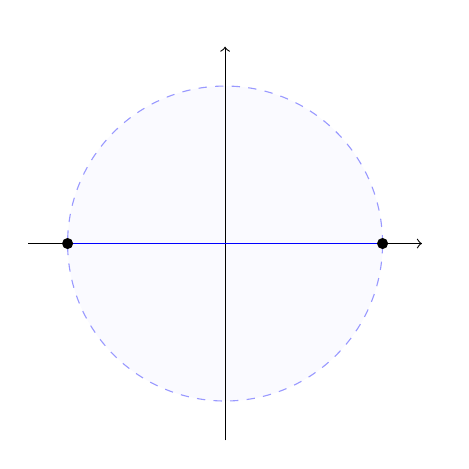
\begin{tikzpicture}
			\coordinate (origin) at (0,0);
			\coordinate (one) at (1.0, 0.0);
			\coordinate (im) at (0.0, 1.0);
		
			\filldraw[dashed, color=blue!40, fill=blue!2] (0, 0) circle (2);

			% draw axes
			\draw [->] (-2.5, 0) -- (2.5, 0) node [right] {$\re$};
			\draw [->] (0, -2.5) -- (0, 2.5) node [above] {$\im$};
		
			\draw [color=blue] (2,0) --(-2, 0);

			% points
			\fill (2,0)  circle[radius=2pt];
			\fill (-2,0)  circle[radius=2pt];
			\end{tikzpicture}
		\caption{$n = 2$} \label{fig:M1}  
	  \end{subfigure}
	  \begin{subfigure}[b]{0.4\linewidth}
		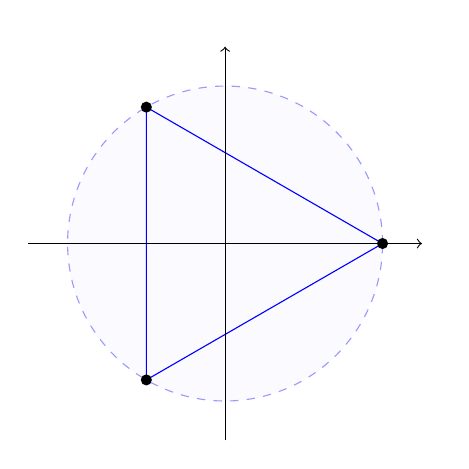
\begin{tikzpicture}
			\coordinate (origin) at (0,0);
			\coordinate (one) at (1.0, 0.0);
			\coordinate (im) at (0.0, 1.0);
			\coordinate (p1) at (2,0);
			\coordinate (p2) at (-1,-1.73206);
			\coordinate (p3) at (-1, 1.73206);
		
			\filldraw[dashed, color=blue!40, fill=blue!2] (0, 0) circle (2);

			\draw [color=blue] (p1) -- (p2) -- (p3) -- (p1);

			% draw axes
			\draw [->] (-2.5, 0) -- (2.5, 0) node [right] {$\re$};
			\draw [->] (0, -2.5) -- (0, 2.5) node [above] {$\im$};
		
			% points
			\fill (p1)  circle[radius=2pt];
			\fill (p2)  circle[radius=2pt];
			\fill (p3)  circle[radius=2pt];
			\end{tikzpicture}%
		\caption{$n = 3$} \label{fig:M2}  
	  \end{subfigure}
	\begin{subfigure}[b]{0.4\linewidth}
		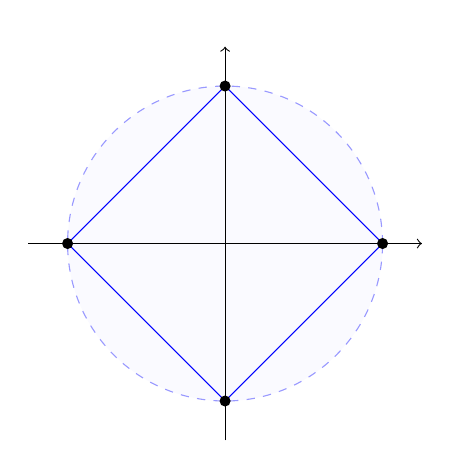
\begin{tikzpicture}
			\coordinate (origin) at (0,0);
			\coordinate (one) at (1.0, 0.0);
			\coordinate (im) at (0.0, 1.0);
			\coordinate (p1) at (2,0);
			\coordinate (p2) at (0,2);
			\coordinate (p3) at (-2,0);
			\coordinate (p4) at (0,-2);
		
			\filldraw[dashed, color=blue!40, fill=blue!2] (0, 0) circle (2);

			\draw [color=blue] (p1) -- (p2) -- (p3) -- (p4) -- (p1);

			% draw axes
			\draw [->] (-2.5, 0) -- (2.5, 0) node [right] {$\re$};
			\draw [->] (0, -2.5) -- (0, 2.5) node [above] {$\im$};
		
			% points
			\fill (p1)  circle[radius=2pt];
			\fill (p2)  circle[radius=2pt];
			\fill (p3)  circle[radius=2pt];
			\fill (p4)  circle[radius=2pt];
			\end{tikzpicture}
	\caption{$n = 4$} \label{fig:M3}  
	\end{subfigure}
	\begin{subfigure}[b]{0.4\linewidth}
		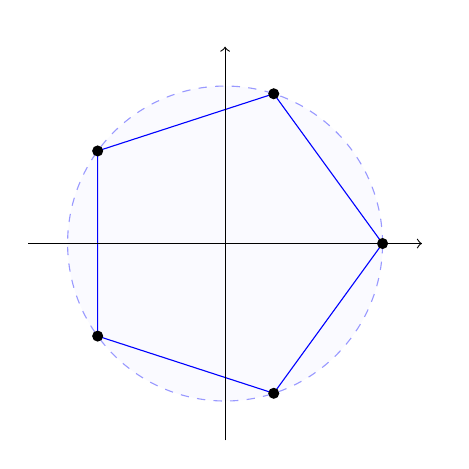
\begin{tikzpicture}
			\coordinate (origin) at (0,0);
			\coordinate (one) at (1.0, 0.0);
			\coordinate (im) at (0.0, 1.0);
			\coordinate (p1) at (2,0);
			\coordinate (p4) at (-1.6180,-1.1756);
			\coordinate (p2) at (0.6180,1.9021);
			\coordinate (p5) at (0.6180,-1.9021);
			\coordinate (p3) at (-1.6180,1.1756);

			\filldraw[dashed, color=blue!40, fill=blue!2] (0, 0) circle (2);

			\draw [color=blue] (p1) -- (p2) -- (p3) -- (p4) -- (p5) -- (p1);

			% draw axes
			\draw [->] (-2.5, 0) -- (2.5, 0) node [right] {$\re$};
			\draw [->] (0, -2.5) -- (0, 2.5) node [above] {$\im$};
		
			% points
			\fill (p1)  circle[radius=2pt];
			\fill (p2)  circle[radius=2pt];
			\fill (p3)  circle[radius=2pt];
			\fill (p4)  circle[radius=2pt];
			\fill (p5)  circle[radius=2pt];
			\end{tikzpicture}
	\caption{$n = 5$} \label{fig:M3}  
	\end{subfigure}
	\caption{$n$th roots of unity on an Argand diagram}
	\end{figure}  

	\begin{proposition}[Geometric Interpretation of Roots of Unity]
		The $n$th roots of unity correspond to the vertices of a regular $n$-gon, inscribed within the unit circle with a vertex at $1$.
	\end{proposition}
	\begin{proof}
		Follows directly from roots of unity written in polar form.
	\end{proof}

\section{Logarithms and Complex Powers}

Over $\R$, the exponential function is one to one. This means that we can quite easily define the inverse function, the logarithm, on the positive reals (the image of the exponential over $\R$).

This is not true over $\C$, as the complex exponential function is many to one. For example, $e^{3\pi i/2} = e^{7 \pi i/2} = -i$. However, we do know that if we have $e^{i\theta} = e^{i \gamma}$, then $\theta$ and $\gamma$ differ by a multiple of $2 \pi$\footnote{This comes from the argument of a complex number only being defined up to a multiple of $2\pi$}. Thus we can define a \emph{multi-valued} logarithm function.

\subsection{The Complex Logarithm}

To see how to define the logarithm over $\C$, let $z$ be any non-zero complex number. Then if we let $\theta = \arg(z)$ with $-\pi < \theta \leq \pi$, then we can write
$$
z = re^{i \theta} =  e^{\log r} e^{i \theta + 2n \pi i} = e^{\log r + i(\theta + 2n \pi)i},
$$
for any $n \in \Z$.

\begin{definition}[Complex Logarithm]
	For a complex number $z$, we define the \vocab{complex logarithm} $\log z$ to be the multi-valued function
	$$
	\log z = \log r + i(\theta + 2n\pi),
	$$
	where $r = |z|$, $\theta = \arg (z)$ with $- \pi < \theta \leq \pi$ and $n \in \Z$.
\end{definition}

\begin{example}[Calculating Complex Logarithms]
	Let $z = \frac{5}{2} + \frac{5\sqrt{3} i}{2}$. We will find $\log z$. We have $|z| = 5$, and the principle value is $\arg(z) = \pi/3$. Thus we have
	$$
	\log z = \log 5 + i (\pi/3 + 2n \pi), \quad n \in \mathbb{Z}.
	$$
\end{example}

Sometimes we will want single-valued behavior from the complex logarithm, and we can define the \vocab{principle logarithm} so that we fix $n = 0$. A warning thou h: if this is done, not all of the familiar properties of the logarithm still hold.\footnote{When taking the principle logarithm, we are really taking a \emph{branch} of the multi-valued logarithm function. This corresponds with taking a slice of the Riemann surface that $\log z$ defines. This gives some weird behavior as we move past certain sets of points (singular points) which breaks many of the identities that we use frequently for the real valued logarithm.}

\subsection{Complex Powers}

The multi-valued nature of the logarithm carries into the notion of taking powers of complex numbers.
For real numbers, we can define $x^a = e^{a \ln x}$ for $x > 0$. We can do the same for complex numbers.

\begin{definition}[Complex Powers]
	We define \vocab{complex powers} for $z, \alpha \in C$ with $z \neq 0$ to be the multi-valued
	$$
	z^{\alpha} = e^{\alpha \log z}.
	$$
\end{definition}

This is not \emph{always} multi valued. For example, if $\alpha \in \Z$, then $z^\alpha$ is unique. If $\alpha \in \Q$, then there will be only finitely many values. However, in most cases there will be infinitely many values.

\begin{example}[Calculating $i^i$]
	We have
	\begin{align*}
		i^i &= e^{i \log i} \\
		&= e^{i \log 1 + i(\pi/2 + 2n\pi)} \\
		&= e^{-(2n + 1/2)\pi},
	\end{align*}
	for any $n \in \Z$. Notably $i^i \in \R$.
\end{example}


\section{Transformations, Lines and Circles}

Consider the following transformations on $\C$.
\begin{itemize}
	\item $z \mapsto z + \alpha$, translation by $\alpha \in \C$.
	\item $z \mapsto \lambda z$, scaling by $\lambda \in \R$,
	\item $z \mapsto e^{i \theta} z$, rotation by $\theta \in \R$. 
	\item $z \mapsto \overline{z}$, reflection in the real axis.
	\item $z \mapsto \frac{1}{z}$, inversion.
\end{itemize}
Using these transformations, we can think geometrically to do things like find equations of various geometric objects.

First we will find the general point on a line
in $\C$ through $z_0$, parallel to $w \in \C$ where $w \neq 0$.
\begin{center}
	\begin{tikzpicture}
		\coordinate (origin) at (0,0);
		\coordinate (one) at (1.0, 0.0);
		\coordinate (im) at (0.0, 1.0);
		\coordinate (z1) at (1, 0.33);
		\coordinate (z2) at (-0.8, 1.4);
	
		% draw axes
		\draw [->] (-1, 0) -- (3.5, 0) node [right] {$\re$};
		\draw [->] (0, -1) -- (0, 2.75) node [above] {$\im$};
	
		% draw vectors
		\draw [->] (origin) -- (z1) node [anchor=south west] {$w$};
		\draw [->] (origin) -- (z2) node [anchor=south west] {$z_0$};
		\draw [<->, dashed, color=blue!80] ($(z2) - (z1)$) -- ($(z2) + (z1) + (z1) + (z1) + (z1) + (z1)$);
		\fill ($(z2) + (z1) + (z1)$)  circle[radius=2pt] node [anchor=south west] {$z$};
	\end{tikzpicture}
\end{center}
We can write $z = z_0 + \lambda w$ for $\lambda \in \R$. To eliminate $\lambda$, we can take the conjugate: $\overline{z} = \overline{z_0} + \lambda \overline{w}$, then $wz - w\overline{z} = \overline{w} z_0 + w \overline{z_0}$.

Similarly, we can find the general point on a circle with a center $c \in \C$ and positive real radius $\rho$.

\begin{center}
	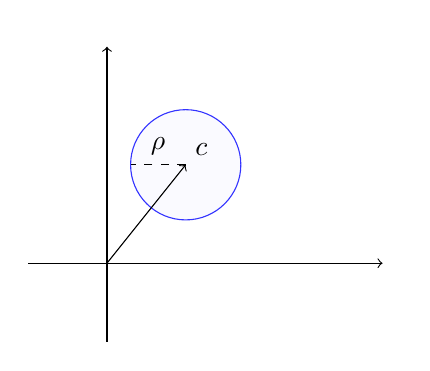
\begin{tikzpicture}
		\coordinate (origin) at (0,0);
		\coordinate (one) at (1.0, 0.0);
		\coordinate (im) at (0.0, 1.0);
		\coordinate (z1) at (1, 1.25);
		% \coordinate (z2) at (-0.8, 1.4);
	
		
		\filldraw[color=blue!80, fill=blue!2] (z1) circle (0.7);

		% draw axes
		\draw [->] (-1, 0) -- (3.5, 0) node [right] {$\re$};
		\draw [->] (0, -1) -- (0, 2.75) node [above] {$\im$};
	
		% draw vectors
		\draw [->] (origin) -- (z1) node [anchor=south west] {$c$};
		\draw [dashed] (1, 1.25) -- (0.3, 1.25) node [pos=0.5, anchor=south] {$\rho$};
		\end{tikzpicture}
\end{center}
A general point on this circle can be written $z = c + \rho e^{i \alpha}$, $\alpha \in \R$. To get rid of $\alpha$, note that we could instead write $|z - c| = \rho$.

We can unify these two forms in the following way.

\begin{proposition}[Circles and Lines in $\C$]
	The equation of any line, and of any circle, may be written respectively as
$$
B z+\bar{B} \bar{z}+C=0 \quad \text { and } \quad z \bar{z}+\bar{B} z+B \bar{z}+C=0
$$
for some complex $B$ and real $C$.

In particular, this is a line in the direction $iB$ or (if $|B|^2 \geq C$), a circle with center $-B$ and radius $\sqrt{|B|^2 - C}$.
\end{proposition}
\begin{proof}[Proof Sketch]
	Do algebra
\end{proof}
